\section{\tool\ Design}
\label{sec:approach}
%\vspace{-2mm}

\begin{figure}
	\centering
		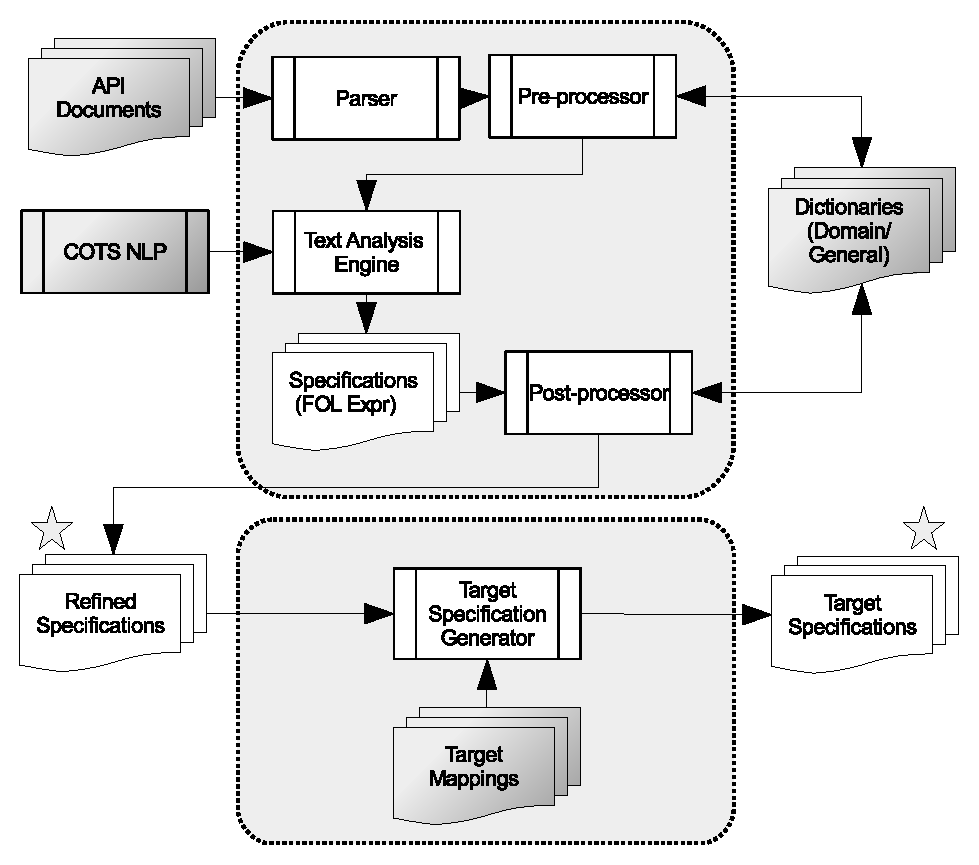
\includegraphics[scale=0.45]{approach.eps}
	\caption{Overview of \tool\ approach}
	\label{fig:approachOverview}
\end{figure}

We next present our approach for inferring specifications from the method descriptions in API Documents.
Figure~\ref{fig:approachOverview} gives an overview of our approach.
Our approach consists of five major components: a preprocessor, a text-analysis engine, a semantic graph generator, specification extractor, and a type analyzer.

The preprocessor accepts API documents and preprocesses the sentences in the method description, such as annotating sentence boundaries and reducing lexical tokens.
The text-analysis engine accepts the pre-processed sentences and annotates them using an NLP parser.
The text-analysis engine further transforms the annotated sentences into the first-order-logic (FOL) representation.
Finally, the specification extractor then leverages the semantic graphs to infer temporal constraints from the FOL representation of a sentence.
Besides the previously described components the approach also consists of a semantic graph generator and type analyzer.
The semantic graph generator accepts the API documents and generates the semantic graphs that are leveraged by specification extractor component.
The type analyzer components infers temporal constraints encoded in the type system of a language by analyzing the API methods parameter and return types.
We next describe each component in detail.


\subsection{Preprocessor}
\label{sub:prep}

The preprocessor accepts the API documents and first extracts method descriptions from it.
In particular, the preprocessor extracts the following fields within method descriptions: 
1) \textit{Summary of the API method},
2) \textit{Summary and type information of parameters of the API method}, 
3) \textit{Summary and type information of return values of the method}, and
4) \textit{Summary and type information of exceptions thrown by the methods}.

This step is required to extract the desired descriptive text from the various presentation styles of the API documents.
In particular, different API documents may have different styles of presenting information to developers.
This difference in style may include the difference in the level of detail presented to the developer.
Our approach thus relies on only basic fields that are trivially available for API methods across different presentation styles. 

After extracting desired information, the natural language text is further preprocessed to be analyzed by subsequent components.
The preprocessing steps are required to increase the accuracy core NLP techniques (described in Section~\ref{sub:CoreNLPback}) that are used in the subsequent phases of \tool\ approach.
In particular, the preprocessor first employs the noun boosting followed by heuristics listed under lexical token reduction, as introduced in Section~\ref{sub:SENLPback}.

Although the previous techniques and heuristics significantly lower the number of lexical tokens in a sentence, some sentences may still contain a considerable number of lexical tokens to overwhelm the POS tagger.
To address this issue, we propose a novel technique (\textit{`Frequent Phrases Reduction'}) to further reduce the number of lexical tokens in a sentence by annotating frequent phrases as a single lexical unit.

In particular, we use n-gram based approach as means to achieve this reduction. 
In the fields of computational linguistics and probability, an n-gram is a contiguous sequence of n words from a given sequence of text or speech. 
We first calculate the most frequently occurring n-grams in the text body. 
In particular, we are interested in the n-grams of length 4 or greater to achieve a reasonable reduction. 
We then prune the list of n-grams based on a subsumption. 
We consider a n-gram of length k ($n_k$) to subsume n-gram of length k-1 ($n_{k-1}$) iff $n_{k-1}$ is a substring of ($n_k$) and the frequency of occurrence of $n_{k-1}$ equals frequency of occurrence of $n_{k}$.
Finally, we rank the list of n-grams based on the frequency of their occurrence in the text, and select top-k n-grams for reduction.
For instance, \textit{Amazon Simple Storage Service}, \textit{an I/O Error Occurs}, and \textit{end of stream} are the examples of such n-grams detected by our approach.
 

%\begin{figure}[t]
%\begin{CodeOut}
%\begin{alltt}
%01: 
%04:
%\end{alltt}
%\end{CodeOut}\vspace*{-2ex}
%\caption{\label{fig:methodAPI} The method description of the \CodeIn{DefineObjectProperty} method in Facebook API}\vspace*{-4ex}
%\end{figure}

\textbf{Prototype Implementation}

Currently our prototype implementation works with online \amazon\ and JDK API. 
However, almost all of the developer documents are provided online as structured webpages.
Thus, current implementation of preprocessor can be easily extended to extract the desired information from any API developer documents.    

Additionally, in current implementation we have manually built the domain dictionaries for the preprocessing using the glossary of terms collected from the websites pertaining to REST and Java API.
We further leveraged the HTML style information in \amazon\ to look for words that were highlighted in code like format. We further leveraged WordNet to maintain a static lookup table of shorthand words to aid named entity handling and abbreviation handling. 

 
Finally, to achieve  n-gram reduction we used Apache Lucene$^{\textregistered}$~\cite{lucene} to achieve.
Apache Lucene is a high-performance, full-featured text search engine library written entirely in Java.
It is a technology suitable for nearly any application that requires full-text search, especially cross-platform.

%Although a POS tagger can be retrained to achieve these pre-processing steps, we prefer annotations to make our approach independent of any specific NLP infrastructure, thus ensuring interoperability with various POS taggers.
	
\subsection{NLP Parser}


The NLP parser accepts the pre-processed documents and annotates every sentence within each document using core NLP techniques described in Section~\ref{sub:CoreNLPback}.
From an implementation perspective, we chose the Stanford parser~\cite{Manning:01}.
However, this component can be implemented using any other existing NLP libraries or approachs.
In particular, we annotate each sentence with POS tags, named-entity Annotations and Stanford-typed dependencies.
For more details on these techniques and their application, please refer to ~\cite{Marneffe06LREC, Marneffe08COLING, pandita12:inferring, pandita13:WHYPER, thummalapentaICSE12}.

%\begin{figure}
%	\centering
%%		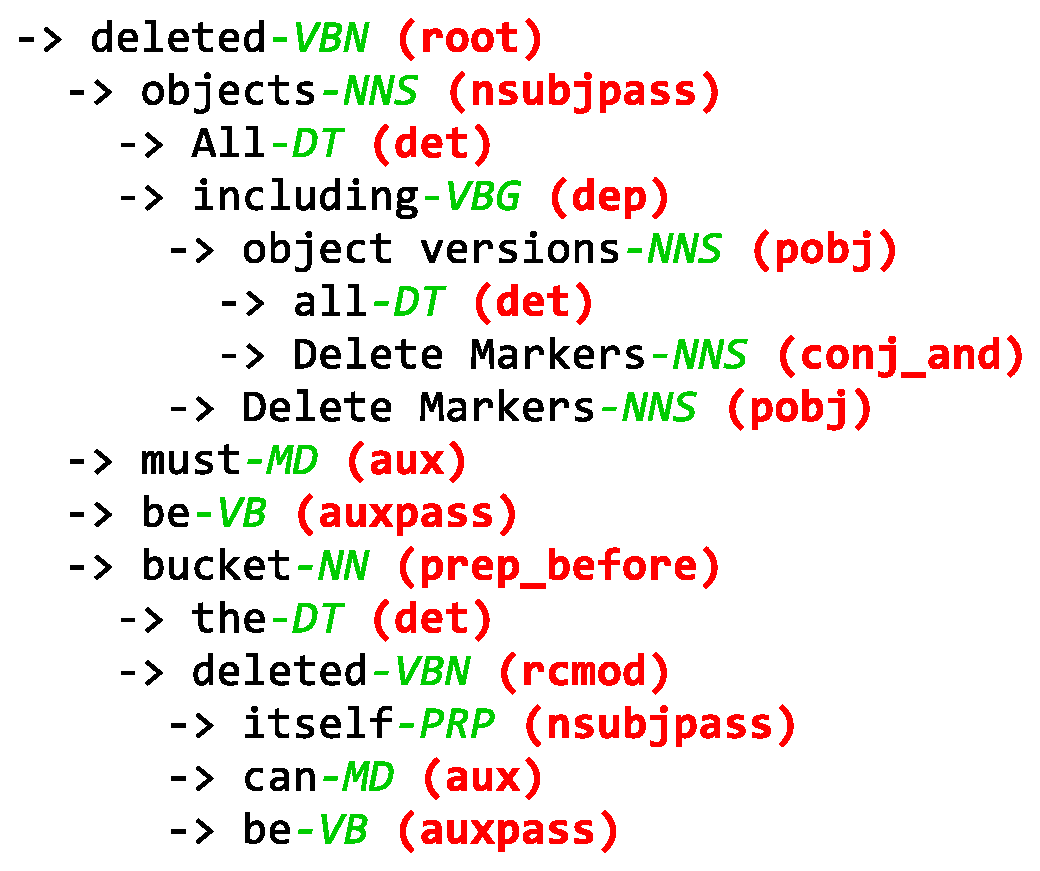
\includegraphics[scale=0.6]{StanfordAnnotated.eps}
%	\caption{Sentence annotated with Stanford dependencies}
%	\label{fig:standep}
%\end{figure}
%
%Next we use an example to illustrate the annotations added by the NLP Parser. Consider the example sentence \textbf{\textit{``Also you can share the yoga exercise to your friends via Email and SMS.''}}, that indirectly refers to the READ\_CONTACTS permission. Figure~\ref{fig:standep} shows the sentence annotated with Stanford-typed dependencies. The words in red are the names of dependencies connecting the actual words of the sentence (in black). Each word is followed by the Part-Of-Speech (POS) tag of the word (in green). For more details on Stanford-typed dependencies and POS tags, please refer to ~\cite{Marneffe06LREC,Marneffe08COLING}.

\subsection{Text Analysis Engine}
\label{sub:TAE}
%
%\begin{figure}
%	\centering
%	%	\includegraphics[scale=0.65]{taeRep.eps}
%	\caption{First-order logic representation of annotated sentence in Figure~\ref{fig:standep}}
%	\label{fig:FOLRep}
%\end{figure}

The text analysis engine component accepts the annotated documents and creates an intermediate representation of each sentence.
We define our representation as a tree structure that is essentially a First-Order-Logic (FOL) expression.
Research literature provides evidence of the adequacy of using FOL for NLP related analysis tasks~\cite{Sinha2009,Sinha2010,pandita12:inferring, pandita13:WHYPER}.

In our representation, every node in the tree except for the leaf nodes is a predicate node. 
The leaf nodes represent the entities.
The children of the predicate nodes are the participating entities in the relationship represented by the predicate.
The first or the only child of a predicate node is the governing entity and the second child is the dependent entity.
Together the governing entity, predicate and the dependent entity node form a tuple.  


As described in Section~\ref{sub:SENLPback} the intermediate representation generation technique is based on the principle of shallow parsing~\cite{Branimir2000}. 
In particular, the intermediate-representation technique is implemented as a function of Stanford-typed dependencies~\cite{Marneffe06LREC,Marneffe08COLING,SNLP,KleinNIPS03}, to leverage the semantic information encoded in Stanford-typed dependencies.


However, we observed that such implementation is overwhelmed by complex sentences.
This limitation mandates the use of additional novel technique of \textit{`Frequent Phrases Reduction'} in preprocessing phase.
We further improve the accuracy of intermediate-representation generation by proposing an hybrid approach, i.e. taking into consideration both the POS tags as well as Stanford-typed dependencies.
The POS tags which annotate the syntactical structure of a sentence are used to further simplify the constituent elements in a sentence. 
We then use the Stanford-typed dependencies that annotate the grammatical relationships between words to construct our FOL representation.
Thus, the intermediate representation generator used in this work is two phase process as opposed to previous work~\cite{pandita12:inferring, pandita13:WHYPER}. 
We next describe these two phases:

\textbf{POS Tags}: We first parse a sentence based on the function of POS tags. 
In particular, we use semantic templates to logically break a sentences into smaller constituent sentences. 
For instance, consider the sentence:

\begin{center}
\scriptsize``All objects (including all object versions and Delete Markers) in the bucket must be deleted before the bucket itself can be deleted.''. \normalsize
\end{center}

The Stanford parser inaccurately annotates the Stanford-typed dependencies of the sentence because of presence of different clauses acting on different subject-object pairs.
We thus break down the sentence into two smaller tractable sentences:

\begin{center}
\scriptsize \textit{``All objects in the bucket must be deleted before the bucket itself can be deleted.}''
	
\textit{``All objects including all object versions and Delete Markers.''}\normalsize 
\end{center} 


Table~\ref{tab:semanticTemplates} shows a list the semantic templates used in this phase.
Column ``Template'' describes conditions where the template is applicable and Column ``Summary'' describes the action taken by our shallow parser when the template is applicable.
All of these semantic templates are publicly available on our project website~\cite{projectweb}.
With respect to the previous example the template no. 3 \textit{( A noun phrase followed by another noun/pronoun/verb phrase in brackets)} is applicable.
Thus our shallow parser breaks the sentence into two individual sentences.
	 
\textbf{Stanford-typed Dependencies}: This phase is equivalent to the intermediate-representation technique described in Section~\ref{sub:SENLPback}.

\subsection{Specification Extractor}
\label{sub:SE}

This component accepts the FOL representation of the sentence.

\begin{itemize}
\item Extracts Specifications from FOL representation. 
\item Specifically looking for modal modifies ``can, could, may, must, should'' 
\item Takes into consideration the negative quantifiers.
\item Algorithm to infer the sequence of operations.
\end{itemize}


\begin{table*}
\begin{center}

\caption{Semantic Templates}
    \begin{tabular}{ | l | p{5cm} |p{10cm} |}
    \hline
    \textbf{S No.} 	& \textbf{Template} & \textbf{Summary} \\ \hline
    
    1. 		& Two sentences joined by a conjunction & Sentence is broken down into two individual sentences with the conjunction term serving as the connector between two. \\ \hline
    2. 		& Two sentences joined by a ``,''& Sentence is broken down to individual independent sentences \\ \hline
    3.		& A noun phrase followed by another noun/pronoun/verb phrase in brackets & Two individual sentences are formed. The first sentence is  the same as the parent sentence sans the noun/pronoun.verb phrase in bracket. The second sentence constitutes of the noun phrase followed by  noun/pronoun/verb phrase without the brackets.\\ \hline
    4.		& A noun phrase by a conditional phrase in brackets & Two individual sentences are formed. The first sentence is the same as the parent sentence sans the conditional phrase in bracket. The second sentence constitutes of noun phrases followed by conditional in the bracket.\\ \hline
    5.		& A conditional phrase followed by a sentence & Two dependent sentences are formed. The first sentence constitutes the conditional phrase. The second sentence constitutes rest of the sentence.\\ \hline
    6.		& A sentence in which the parent verb phrase is over two child verb phrases joined by a conjunction & Two dependent sentences are formed where the dependency is the conjunction. The first sentence is formulated by removing conjunction and second child verb phrase. The second sentence is formulated by removing conjunction and first child verb phrase. \\ \hline
    \end{tabular}
	\label{tab:semanticTemplates}
\end{center}
\end{table*}


\subsection{Semantic-Graph Generator}
\label{sub:ACA}

A key way of identifying reference to a method within the API in our proposed approach is the employment of a semantic graph of an API.
In particular, we propose to initially infer such graphs from API documents.
Manually creating a semantic graph is prohibitively time consuming and may be error prone.
We thus employ a systematic methodology (proposed previously in ~\cite{pandita13:WHYPER}) to infer such semantic graphs from API documents that can potentially be automated.
We first consider the name of the class.
We then find the synonyms terms used refer to the class in question.
The synonym terms are listed as by breaking down the camel-case notation in the class name.
This list is further augmented by listing the name of the parent classes and implemented interfaces if any. 

\begin{figure}
	\centering
		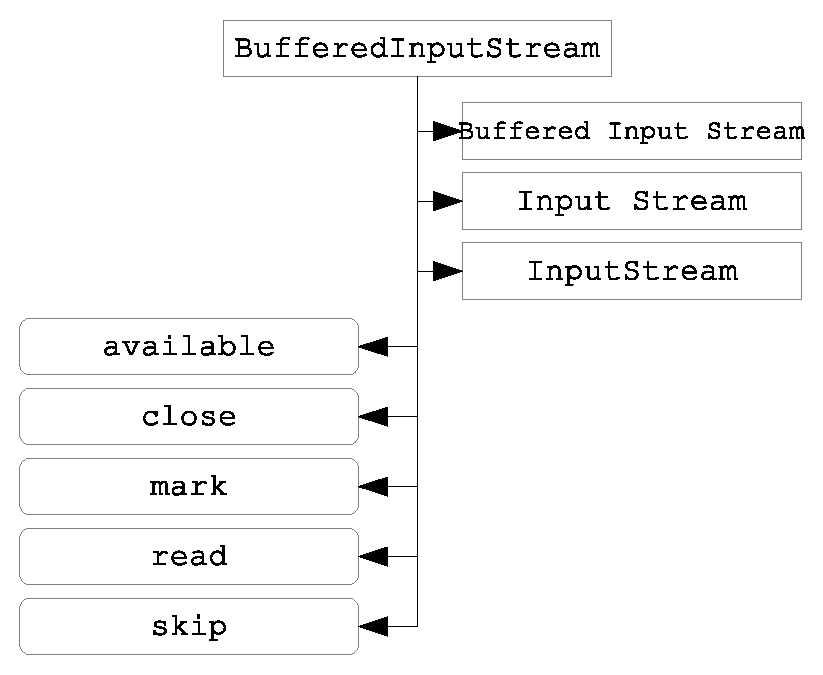
\includegraphics[scale=0.4]{KnowledgeGraph.eps}
	\caption{Semantic Graph for the \CodeIn{BufferedInputStream} class in Java}
	\label{fig:knowledge}
\end{figure} 


We then systematically inspect the member methods to identify actions applicable to the objects represented by the class. From the name of a public method (describing a possible action on the object), we extract verb phrases. The verb phrases are used as the associated actions applicable on the object. For instance, \CodeIn{BufferedInputReader} defines operations available, close, mark, and so on. We associate these operations with the objects of type \CodeIn{BufferedInputReader}. Figure~\ref{fig:knowledge} shows a sub-graph of  graph for \CodeIn{BufferedInputReader} class. The phrases in solid rectangles are synonyms of the class name \CodeIn{BufferedInputReader}. The phrases in rounded rectangle are the actions applicable on \CodeIn{BufferedInputReader} class.
  


\algsetup{indent=1em}
\begin{algorithm}[t!]
\begin{algorithmic}[1]
\begin{scriptsize}
\REQUIRE K\_Graph $g$, FOL\_rep $rep$ 
\ENSURE String $action$
\STATE $String\ action\ =\ \phi$
\STATE $List\ r\_name\_list\ =\ g.resource\_Names$
\STATE $FOL\_rep\ r'\ =\ rep.findLeafContaining(r\_nam\_list)$
\STATE $List\ actionList\ =\ g.actionList$
\WHILE{$(r'.hasParent)$}
	\IF{$actionList.contains(r'.parent.predicate)$}
		\STATE $action\ =\ actionList.matching(r'.parent.predicate)$
		\STATE $break$
	\ELSE
		\IF{$actionList.contains(r'.leftSibling.predicate)$}
			\STATE $action\ =\ actionList.matching(r'.leftSibling.predicate)$
			\STATE $break$
		\ENDIF
	\ENDIF
	\STATE $r'\ =\ r'.parent$
\ENDWHILE
\RETURN $action$
\end{scriptsize}
\end{algorithmic}
\caption{Action\_Extractor}
\label{alg:SenAnnotaator}
\end{algorithm} 


\begin{algorithm}[t!]
\begin{algorithmic}[1]
\begin{scriptsize}
\REQUIRE List $methodList$ 
\ENSURE Graph $seq\_Graph$
\STATE $Graph\ seq\_Graph\ =\ \phi$
\STATE $Map\ idx\ = createIdx(methodList)$

\FORALL{$Method\ mtd\ in\ methodList$} 
	\STATE $seq\_Graph.addVertex(mtd)$
\ENDFOR

\FORALL{$Method\ mtd\ in\ methodList$} 
	\IF{$mtd.isPublic()$}
		\IF{$!mtd.isStatic()$}
			\STATE $List\ preList\ =\ idx.query(mtd.declaringType)$
			\FORALL{$Method\ mtd'\ in\ preList$}
				\STATE $seq\_Graph.addEdge(mtd',mtd)$
			\ENDFOR
		\ENDIF
		\FORALL{$Parameter\ param\ in\ mtd.getParameters()$}
			\IF{$!isBasicType(param.Type)$}
				\STATE $List\ preList\ =\ idx.query(paramType)$
				\FORALL{$Method\ mtd'\ in\ preList$}
					\STATE $seq\_Graph.addEdge(mtd',mtd)$
				\ENDFOR				
			\ENDIF
		\ENDFOR
	\ENDIF
\ENDFOR
\RETURN $seq\_Graph$
\end{scriptsize}
\end{algorithmic}
\caption{Type\_Sequence\_Builder}
\label{alg:SeqAnnotaator}
\end{algorithm} 



%The FOL representation helps us effectively deal with the problem of \emph{confounding effects} of keywords as described in Section~\ref{sec:overview}. In particular, the FOL assists in distinguishing between a resource that would be a leaf node and an action that would be a predicate node in the intermediate representation of a sentence. The generated FOL representation of the sentence is then provided as an input to the semantic engine for further processing.
%
%
%
%\subsection{Semantic Engine (SE)}
%\label{sub:SE}
%The Semantic Engine (SE) accepts the FOL representation of a sentence and based on the semantic graphs of Android permissions annotates a sentence if it matches the criteria. A semantic graph is basically a semantic representation of the resources which are governed by a permission. For instance, the READ\_CONTACTS permission governs the resource ``CONTACTS'' in Android system.
%
%
%Figure~\ref{fig:knowledge} shows the semantic graph for the permission READ\_CONTACTS. A semantic graph primarily constitutes of subordinate resources of a permission (represented in rectangular boxes) and a set of available actions on the resource itself (represented in curved boxes). Section~\ref{sub:ACA} elaborates on how we build such graphs systematically.
%
%Our SE accepts the semantic graph pertaining to a permission and annotates a sentence based on the algorithm shown in Algorithm~\ref{alg:SenAnnotaator}. The Algorithm accepts the FOL representation of a sentence $rep$, the semantic graph associated with the resource of a permission $g$ and a boolean value $recursion$ that governs the recursion. The algorithm outputs a boolean value $isPStmt$, which is \CodeIn{true} if the statement describes the permission associated with a semantic graph ($g$), otherwise \CodeIn{false}. 
%
%Our algorithm systematically explores the FOL representation of the sentence to determine if a sentence describes the need for a permission. First, our algorithm attempts to locate the occurrence of associated resource name within the leaf node of the FOL representation of the sentence (Line 3). The method \CodeIn{findLeafContaining(name)} explores the FOL representation to find a leaf node that contains term \CodeIn{name}. Furthermore, we use WordNet and Lemmatisation~\cite{Do09:Robust} to deal with synonyms of a word in question to find appropriate matches. Once a leaf node is found, we systematically traverse the tree from the leaf node to the root, matching all parent predicates as well as immediate child predicates [Lines 5-16].
%
%Our algorithm matches each of the traversed predicate with the actions associated with the resource defined in semantic graph. Similar to matching entities, we also employ WordNet and Lemmatisation~\cite{Do09:Robust} to deal with synonyms to find appropriate matches. If a match is found, then the value \CodeIn{isPStmt} is set to  \CodeIn{true}, indicating that the statement describes a permission.
%
%In case no match is found, our algorithms recursively search all the associated subordinate resources in the semantic graph of current resource. A subordinate resource may further have its own subordinate resources. Currently, our algorithm considers only immediate subordinate resources of a resource to limit the false positives.
%
%%We limit the exploration to depth 1 to limit the false positives. That means only immediate subordinate resources of a resource will be explored.
%
%In the context of the FOL representation shown in Figure~\ref{fig:FOLRep}, we invoke Algorithm~\ref{alg:SenAnnotaator} with the semantic graph shown in Figure~\ref{fig:knowledge}. Our algorithm attempts to find a leaf node containing term ``CONTACT'' or some of its synonym. Since the FOL representation does not contain such a leaf node, algorithm calls itself with semantic graphs of subordinate resources (Line 17-25), namely `NUMBER', `EMAIL', `LOCATION', `BIRTHDAY', `ANNIVERSARY'. 
%
%The subsequent invocation will find the leaf-node ``email'' (annotated 9 in Figure~\ref{fig:FOLRep}). Our algorithm then explores the preceding predicates and finds predicate ``share'' (annotated 2 in Figure~\ref{fig:FOLRep}). The Algorithm matches the word ``share'' with action ``send'' (using Lemmatisation and WordNet similarity), one of the actions available in the semantic graph of resource `EMAIL' and returns \CodeIn{true}. Thus, the sentence is appropriately identified as describing the need for permission READ\_CONTACT. 
%
%

